%===============================================================================
\subsubsection*{a)}
%===============================================================================

\code{SimplePathIntegrator::Li} is quite involved. It's entire implementation is seen in Listing \ref{lst:simple-path-integrator}. First, we copy \code{cameraRay}. Since \code{ray} will change after bounces, we need a copy that we can modify. We also declare two variables \code{radiance}, which stores the sum of outgoing light of each intersection point that we find on our path. \code{throughput} on the other hand stores the incomming light. Then, we can iterate with a simple \code{for}-loop, which iterates at maximum \code{m\_maxBounces} times. Then these steps are done in order:

{
\renewcommand{\labelenumi}{\arabic{enumi}.}
\begin{enumerate}
\item
We check if we hit something. If not, we evaluate the environment. Since we can't compute another bounce, we simply break out of the \code{for}-loop.

\item
Then we check if we hit an emitter. If so, evaluate it and add it to \code{radiance}. It's weighted by \code{throughput}, the incomming light of the previous bounces.

\item
Then we compute $\omega_i$, $\omega_o$ and the PDF. $\omega_i$ is just the inverse ray we just traveled, $\omega_o$ is randomly determined using \code{Warp::squareToUniformHemisphere}, and we get the PDF using \code{Warp::squareToUniformHemispherePdf}, which should be $\frac{1}{2\pi}$. In any case, if it return a negative, we break out of the \code{for}-loop.

\item
Then we evaluate the bsdf and store it in \code{throughput}.

\item
Finally we produce a new ray. It's simply the random $\omega_o$ direction we computed earlier, from which we construct a ray, whose origin is the intersection point.

\end{enumerate}
}

%===============================================================================
\subsubsection*{b)}
%===============================================================================

\begin{figure}[htbp]
    \centering
    \begin{subfigure}{0.32\textwidth}
        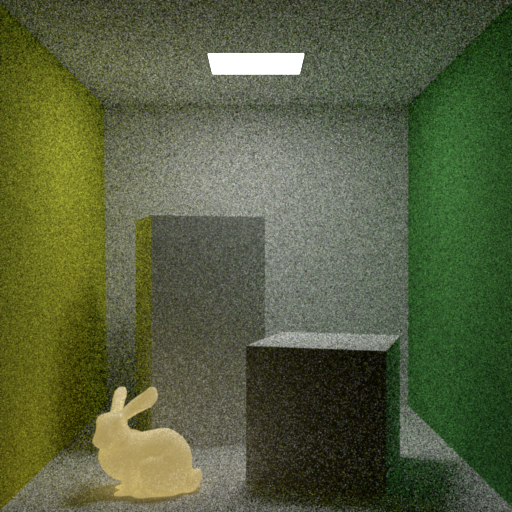
\includegraphics[width=\linewidth]{pictures/cbox-path-512spp-ref.png}
    \end{subfigure}
    \hfill
    \begin{subfigure}{0.32\textwidth}
        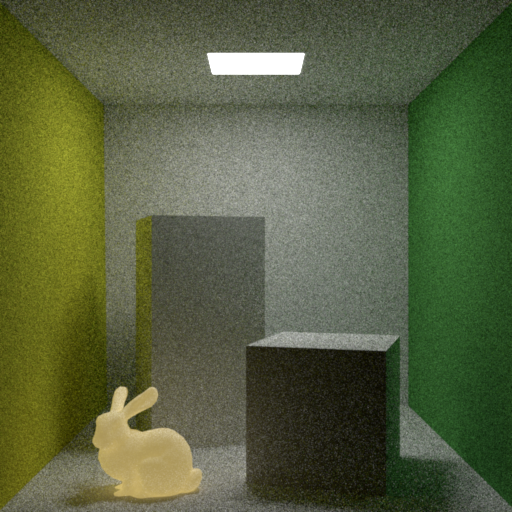
\includegraphics[width=\linewidth]{pictures/cbox-path.png}
    \end{subfigure}
    \hfill
    \begin{subfigure}{0.32\textwidth}
        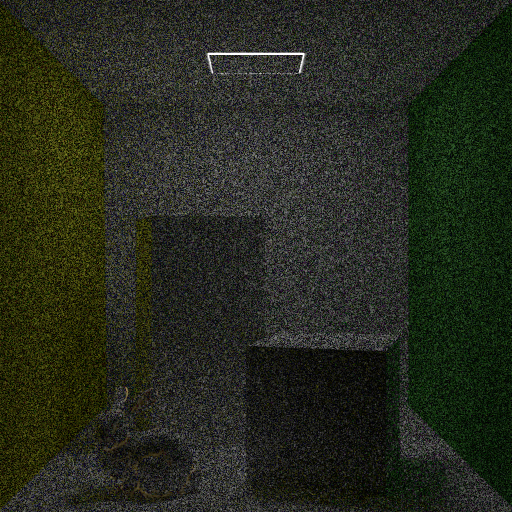
\includegraphics[width=\linewidth]{pictures/compare_3_2.png}
    \end{subfigure}
    \caption{The reference image (left) and our result (center) compared (right). Our result was rendered using 1024 samples. To us the pictures look identical, but the noise is different. We assume due to the reference image being older, or because we used more samples, the RNG is seeded differently, resulting int completely different noise.}
    \label{fig:comparison-3-2}
\end{figure}

\newpage

\begin{lstlisting}[caption={\code{SimplePathIntegrator::Li}},label={lst:simple-path-integrator}]
Color3f Li(const Scene *scene, Sampler *sampler, const Ray3f &cameraRay) const override {
    // cached values between bounces
    Ray3f ray = cameraRay;
    Color3f radiance {0.0f};
    Color3f throughput {1.0f};
    
    // iterate bounces
    for (int i = 0; i < m_maxBounces; ++i) {
        
        // 1. check if we hit something
        Intersection its;
        if (!scene->rayIntersect(ray, its)) {
            // nothing hit! evaluate environment and stop bouncing
            auto emitter = scene->getEnvironmentMap();
            if (emitter) {
                radiance += throughput * emitter->eval(-ray.d);
            }
            
            break;
        }
        
        // 2. if emitter, evaluate and add to radiance
        auto emitter = its.mesh->getEmitter();
        if (emitter) {
            radiance += throughput * emitter->eval(its.toLocal(-ray.d));
        }
        
        // 3. compute wi, wo and pdf
        auto wi = its.toLocal(-ray.d);
        auto wo = Warp::squareToUniformHemisphere(sampler->next2D());
        float pdf = Warp::squareToUniformHemispherePdf(wo);
        if (pdf <= 0.0f) {
            break;
        }
        
        // 4. evaluate bdsf
        BSDFQueryRecord bRec(wi, wo, ESolidAngle, its.uv);
        auto bsdf = its.mesh->getBSDF()->eval(bRec);
        float cosine = Frame::cosTheta(wo);
        if (cosine <= 0.0f) {
            break;
        }
        
        throughput *= bsdf * (cosine / pdf);
        
        // 5. compute new ray
        auto worldDirection = its.toWorld(wo);
        worldDirection.normalize();
        ray = Ray3f{its.p, worldDirection};
    }
    
    return radiance;
}
\end{lstlisting}